\documentclass[9pt]{beamer}

\beamertemplatenavigationsymbolsempty
\renewcommand\mathfamilydefault{cmr}

\usepackage{pajmath}
\usepackage{booktabs}
\usepackage{colortbl}

\usepackage{tikz}
\usetikzlibrary{positioning,shapes.misc,calc,backgrounds,scopes} 
\usetikzlibrary{datavisualization}
\usetikzlibrary{datavisualization.formats.functions}
\tikzset{boxed/.style={
  thick,
  draw=black,
  top color=white,
  text height=1.5ex,
  text depth=.25ex
}}


\newcommand\lo{$-1$}
\newcommand\hi{$\phan1$}
\newcommand\ze{$\phan0$}
\newcommand\Ze{$\phan\Vzero$}
\newcommand\pskip{\pause\bigskip}
\newcommand\lspace{\addtolength{\itemsep}{0.5\baselineskip}}
\newcommand\red[1]{{\color{red}#1}}

\title{Reinforcement Learning:\\$Q$-learning and Tic-Tac-Go}
\author{BIOE 498/598 PJ}
\date{Spring 2021}

\begin{document}
\frame{\titlepage}


\begin{frame}{Review}

\begin{itemize}\lspace
	\item Discount factors shorten the horizon of RL problems, causing the agent to focus on rewards in the near future.
	\item Temporal Difference (TD) learning incrementally updates value functions using a new experience.
	\item Learning $Q$-factors eliminates the need to predict the next state given an action; however, the number of $Q$-factors is much greater than the number of states.
	\item<2-> \textbf{Today:}
		\begin{itemize}\lspace
			\item Review SARSA
			\item $Q$-learning
			\item Tic-Tac-Go
		\end{itemize}
\end{itemize}
	
\end{frame}

\begin{frame}{Learning $Q$-factors}

Using $Q$-factors, the policy problem at state~$s_i$
	\[ \max_{a} \mathbb{E}\left\{ r_i + \gamma V(s_{i+1}) \right\} \]
becomes
	\[ \max_{a} \mathbb{E}\left\{ Q(s_i,a) \right\}. \]

\pskip
\begin{itemize}
	\item \textbf{Pro:} We do not need a model or a way to predict $s_{i+1}$.
	\item \textbf{Con:} We need to learn a $Q$-factor for every state/action pair.
\end{itemize}

\pskip
We can learn $Q$-factors using a TD approach given a trajectory $s_0,a_0,r_0$, $s_1,a_1,r_1$ $\ldots$, $s_T,r_T$:
\begin{align*}
	\hat{Q}(s_i,a_i) &= r_i + \gamma Q(s_{i+1},a_{i+1}) & \text{target} \\
	Q(s_i,a_i) &\leftarrow Q(s_i,a_i) + \alpha\left[ \hat{Q}(s_i,a_i) - Q(s_i,a_i) \right] & \text{update}
\end{align*}
This approach is called \emph{SARSA}.

\end{frame}

\begin{frame}{SARSA follows a trajectory, not an optimal path}

The SARSA update equation is

\[ Q(s_i,a_i) \leftarrow Q(s_i,a_i) + \alpha\bigg[ \underbrace{r_i + \gamma Q(s_{i+1},a_{i+1})}_\text{target} - Q(s_i,a_i) \bigg]. \]

\pskip
Our estimate of $Q(s_i,a_i)$ is based on
\begin{itemize}
	\item The reward $r_i$ experienced by selecting action $a_i$ in state $s_i$.
	\item The future reward $Q(s_{i+1},a_{i+1})$ based on the action $a_{i+1}$ from the trajectory.
\end{itemize}

\pskip
The policy that generated the trajectory is not optimal, so it is likely that $a_{i+1}$ was not the best action to take.

\bigskip
Selecting a suboptimal action underestimates the reward to go, and therefore the value $Q(s_i,a_i)$.

\end{frame}

\begin{frame}{$Q$-learning}

The $Q$-learning algorithm changes the SARSA update
\[ Q(s_i,a_i) \leftarrow Q(s_i,a_i) + \alpha\left[ r_i + \gamma Q(s_{i+1},a_{i+1}) - Q(s_i,a_i) \right] \]
to use the optimal action in state $s_{i+1}$:
\[ Q(s_i,a_i) \leftarrow Q(s_i,a_i) + \alpha\left[ r_i + \gamma\, \red{\max_a Q(s_{i+1},a)} - Q(s_i,a_i) \right]. \]
	
\pskip
$Q$-learning can converge faster to an optimal policy. However, it has two drawbacks:
\begin{enumerate}
	\item If the number of available actions is large, the maximization operator can be expensive to evaluate.
	\item The maximization operator is biased.
\end{enumerate}
\end{frame}

\begin{frame}{Records were meant to be broken.}

\begin{itemize}\lspace
	\item Imagine that the quality of professional basketball players was fixed over time.
	\item In this case, scoring records would still be broken.
	\item Basketball includes stochastic elements, so as more games are played the chance of observing outliers increases.
\end{itemize}

\pskip
Any algorithm with a $\max$ operator will drift upwards over time, \emph{even if the mean value remains fixed}.

\bigskip
For $Q$-learning, we need to combat the bias in the $\max$ operator.
	
\end{frame}

\begin{frame}{Double $Q$-learning}

One solution to the $\max$ bias is using two separate $Q$ functions (networks), called $Q_1$ and $Q_2$.

\bigskip
Both $Q_1$ and $Q_2$ are trained with separate experiences. (Or, one network can \emph{lag} behind the other in experiences.)

\pskip
When updating, we use one network to select the action, and the other network to compute its value.
\begin{align*}
	Q_1(s_i,a_i) &\leftarrow Q_1(s_i,a_i) + \alpha\left[ r_i + \gamma\, Q_2(s_{i+1},a_1) - Q_1(s_i,a_i) \right] \\
	& \quad a_1 \equiv \arg\max_a Q_1(s_{i+1},a) \\ \\
	Q_2(s_i,a_i) &\leftarrow Q_2(s_i,a_i) + \alpha\left[ r_i + \gamma\, Q_1(s_{i+1},a_2) - Q_2(s_i,a_i) \right] \\
	& \quad a_2 \equiv \arg\max_a Q_2(s_{i+1},a)
\end{align*}

\pskip
Even if $a_1$ was selected because $Q_1(s_{i+1},a_1)$ was aberrantly high, the value $Q_2(s_{i+1},a_1)$ will not share this bias.
	
\end{frame}

\begin{frame}{Deep $Q$-learning}

\begin{itemize}\lspace
	\item Currently, the most common method for approximating $Q$-factors is \emph{deep learning} with artificial neural networks.
	\item We're going to learn to play a simple board game called Tic-Tac-Go.
	\item We want a game that is simple enough to be computationally tractable, but not easily solved.
	\item<2->Tic-Tac-Toe is simple, but solved. If both players follow an optimal strategy, the game will always end in a draw.
	\item<3->Go is unsolved, but approximating $Q$-factors is ridiculously expensive.
\end{itemize}

\end{frame}

\begin{frame}{Tic-Tac-Go}

\begin{columns}
\begin{column}{0.6\textwidth}

\begin{itemize}\lspace
	\item Tic-Tac-Go is played on a $4\times4$ grid.
	\item Before playing, $4$ squares are randomly ``blocked''.
	\item Two players, \texttt{X} and \texttt{O}, alternate placing pieces in open squares.
	\item Players receive points for making horizontal or vertical ``chains''.
	\item A chain of length $k$ is worth $(k-1)^2$ points.
		\begin{align*}
			\text{length } 2 &= 1 \text{ point} \\
			\text{length } 3 &= 4 \text{ points} \\
			\text{length } 4 &= 9 \text{ points} \\	
		\end{align*}

\end{itemize}

\end{column}

\begin{column}{0.4\textwidth}
	\begin{center}
		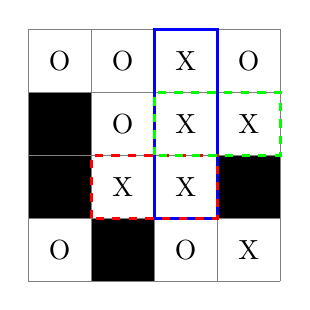
\begin{tikzpicture}[scale=0.8]
			\draw [thin,gray] (0,0) grid (4,4);
			\filldraw [fill=black,draw=gray] 
						  (0,1) rectangle (1,2)
						  (0,2) rectangle (1,3)
						  (1,0) rectangle (2,1)
						  (3,1) rectangle (4,2);
			\onslide<2->{
				\draw (0.5,3.5) node {O}
					  (1.5,3.5) node {O}
					  (1.5,2.5) node {O}
					  (0.5,0.5) node {O}
					  (2.5,0.5) node {O}
					  (3.5,3.5) node {O}
					  (2.5,1.5) node {X}
					  (2.5,2.5) node {X}
					  (2.5,3.5) node {X}
					  (1.5,1.5) node {X}
					  (3.5,0.5) node {X}
					  (3.5,2.5) node {X};
			}
			\onslide<3->{
				\draw [blue,very thick] (2,1) rectangle (3,4);
				\draw [red,very thick,dashed] (1,1) rectangle (3,2);
				\draw [green,very thick,dashed] (2,2) rectangle (4,3);
			}
		\end{tikzpicture}
		
		\onslide<3->{
			\bigskip
			\texttt{X} score: $(2-1)^2 + (2-1)^2 + (3-1)^2 = 6$
			
			\bigskip
			\texttt{O} score: \\$(2-1)^2 + (2-1)^2 = 2$
		}
	\end{center}	
\end{column}
\end{columns}
	
\end{frame}

\begin{frame}{States for Tic-Tac-Go}

\begin{itemize}
	\item States $s_i$ are configurations of the board.
	\item Each of the 16 squares can be empty, blocked, \texttt{X}, or \texttt{O}.
	\item There are $_{16}C_4 \times 3^{12} = 967,222,620$ possible board configurations.
	\item Each configuration has, on average, $6$ possible moves, so there are more than $5.8\times10^{9}$ $Q$-factors to learn!
\end{itemize}

\pskip
How do we encode the states for a function approximator?

\end{frame}

\begin{frame}{Option 1: Ignore the blocked states, $-1$, $0$, $+1$}

\begin{columns}
\begin{column}{0.6\textwidth}

\begin{itemize}\lspace
	\item Let's ignore the blocked squares since we can't play on them.
	\item A square with \texttt{X} is $-1$, \texttt{0} is $+1$, and empty squares are $0$.
	\item Each state $s_i$ is a $12\times1$ trinary vectory.

\end{itemize}

\end{column}

\begin{column}{0.4\textwidth}
	\pause
	\begin{center}
		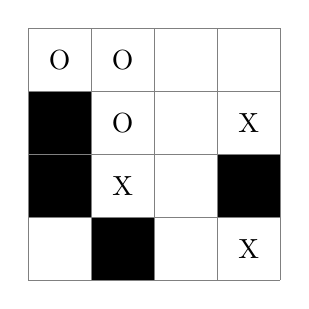
\begin{tikzpicture}[scale=0.8]
			\draw [thin,gray] (0,0) grid (4,4);
			\filldraw [fill=black,draw=gray] 
						  (0,1) rectangle (1,2)
						  (0,2) rectangle (1,3)
						  (1,0) rectangle (2,1)
						  (3,1) rectangle (4,2);
			\draw (0.5,3.5) node {O}
				  (1.5,3.5) node {O}
				  (1.5,2.5) node {O}
				  (1.5,1.5) node {X}
				  (3.5,0.5) node {X}
				  (3.5,2.5) node {X};
		\end{tikzpicture}
		
		\bigskip
		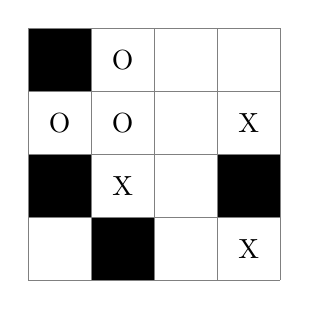
\begin{tikzpicture}[scale=0.8]
			\draw [thin,gray] (0,0) grid (4,4);
			\filldraw [fill=black,draw=gray] 
						  (0,1) rectangle (1,2)
						  (0,3) rectangle (1,4)
						  (1,0) rectangle (2,1)
						  (3,1) rectangle (4,2);
			\draw (0.5,2.5) node {O}
				  (1.5,3.5) node {O}
				  (1.5,2.5) node {O}
				  (1.5,1.5) node {X}
				  (3.5,0.5) node {X}
				  (3.5,2.5) node {X};
		\end{tikzpicture}

	\end{center}	
\end{column}
\end{columns}
	
\end{frame}

\begin{frame}{Option 2: One-hot encoding}

\begin{columns}

\begin{column}{0.3\textwidth}
	\begin{center}
		state
		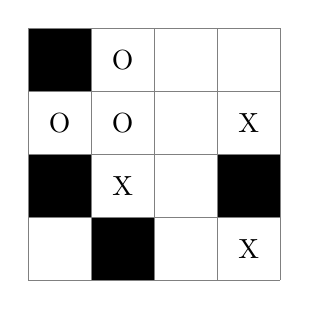
\begin{tikzpicture}[scale=0.8]
			\draw [thin,gray] (0,0) grid (4,4);
			\filldraw [fill=black,draw=gray] 
						  (0,1) rectangle (1,2)
						  (0,3) rectangle (1,4)
						  (1,0) rectangle (2,1)
						  (3,1) rectangle (4,2);
			\draw (0.5,2.5) node {O}
				  (1.5,3.5) node {O}
				  (1.5,2.5) node {O}
				  (1.5,1.5) node {X}
				  (3.5,0.5) node {X}
				  (3.5,2.5) node {X};
		\end{tikzpicture}	
		\onslide<2->{
			\bigskip
			
			Each state is a \\$16\times4$ matrix \\or a \\$64\times1$ vector.
		}
	\end{center}
\end{column}

\begin{column}{0.3\textwidth}
	\begin{center}
		blocked
		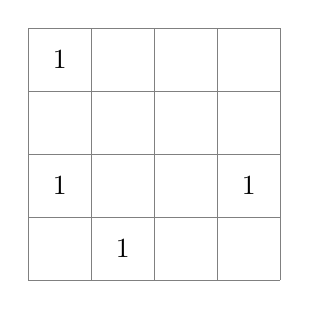
\begin{tikzpicture}[scale=0.8]
			\draw [thin,gray] (0,0) grid (4,4);
			\draw (0.5,1.5) node {1}
				  (0.5,3.5) node {1}
				  (1.5,0.5) node {1}
				  (3.5,1.5) node {1};
		\end{tikzpicture}
		\bigskip
		
		empty
		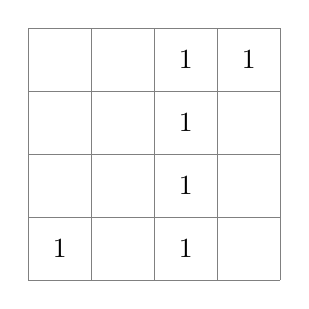
\begin{tikzpicture}[scale=0.8]
			\draw [thin,gray] (0,0) grid (4,4);
			\draw (0.5,0.5) node {1}
				  (2.5,0.5) node {1}
				  (2.5,1.5) node {1}
				  (2.5,2.5) node {1}
				  (2.5,3.5) node {1}
				  (3.5,3.5) node {1};
		\end{tikzpicture}	
	\end{center}
\end{column}

\begin{column}{0.3\textwidth}
	\begin{center}
		player \texttt{O}
		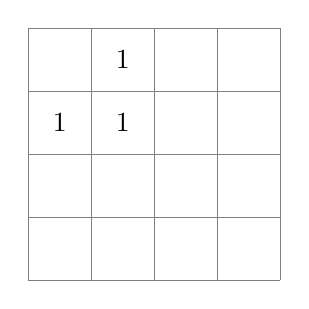
\begin{tikzpicture}[scale=0.8]
			\draw [thin,gray] (0,0) grid (4,4);
			\draw (0.5,2.5) node {1}
				  (1.5,3.5) node {1}
				  (1.5,2.5) node {1};
		\end{tikzpicture}
		\bigskip
		
		player \texttt{X}
		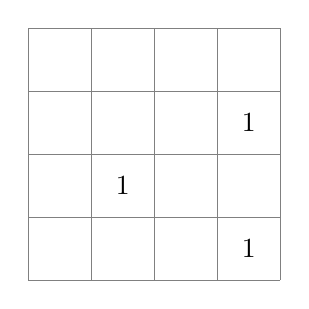
\begin{tikzpicture}[scale=0.8]
			\draw [thin,gray] (0,0) grid (4,4);
			\draw (1.5,1.5) node {1}
				  (3.5,0.5) node {1}
				  (3.5,2.5) node {1};
		\end{tikzpicture}	
	\end{center}
\end{column}
	
\end{columns}

\end{frame}

\begin{frame}{Our plan for Tic-Tac-Go}

\begin{itemize}\lspace
	\item We'll start with a one-hot encoding, as it simplifies the neural network.
	\item The four features are not independent, but we leave them to accelerate learning.
	\item However, \emph{state unrolling} loses spatial information about the board. We will eventually avoid unrolling via \emph{convolution}.
	\item Convolution will also exploit symmetry in the game board.
\end{itemize}
	
\end{frame}

\begin{frame}{Summary}

\begin{itemize}\lspace
	\item $Q$-learning is a state-of-the-art technique for RL.
	\item Double $Q$-learning counteracts the bias in the $\max$ operator.
	\item Defining the state space for simple board games in not trivial. Some state space representations are better for learning.
	\item<2-> \textbf{Next time:} Artificial neural networks.
\end{itemize}
	
\end{frame}


\end{document}
